\documentclass{beamer}
 
\usepackage[utf8]{inputenc}
\usepackage{graphicx}
\usepackage{subcaption}
\graphicspath{ {images/} }

\usetheme{metropolis} 
 
%Information to be included in the title page:
\title{Relative Changes in removal of constraints in 3D Sudokus}
\author{Samarth Bhargav, Alexander Geenen}
\institute{University of Amsterdam}
\date{\today}
 
\AtBeginSection[]
{
	\begin{frame}
		\frametitle{Table of Contents}
		\tableofcontents[currentsection]
	\end{frame}
}
 
 
\begin{document}
 
\frame{\titlepage}


\begin{frame}[standout]
Video: https://youtu.be/dTnoKvseOFI \\
Github Link: https://github.com/samarthbhargav/constraint-removal-3d-sudoku
\end{frame}
 
\begin{frame}
	\frametitle{Table of Contents}
	\tableofcontents
\end{frame}

\section{Introduction}  


\begin{frame}
\frametitle{Example}
\begin{figure}
	\centering
	\begin{subfigure}[b]{0.4\textwidth}
		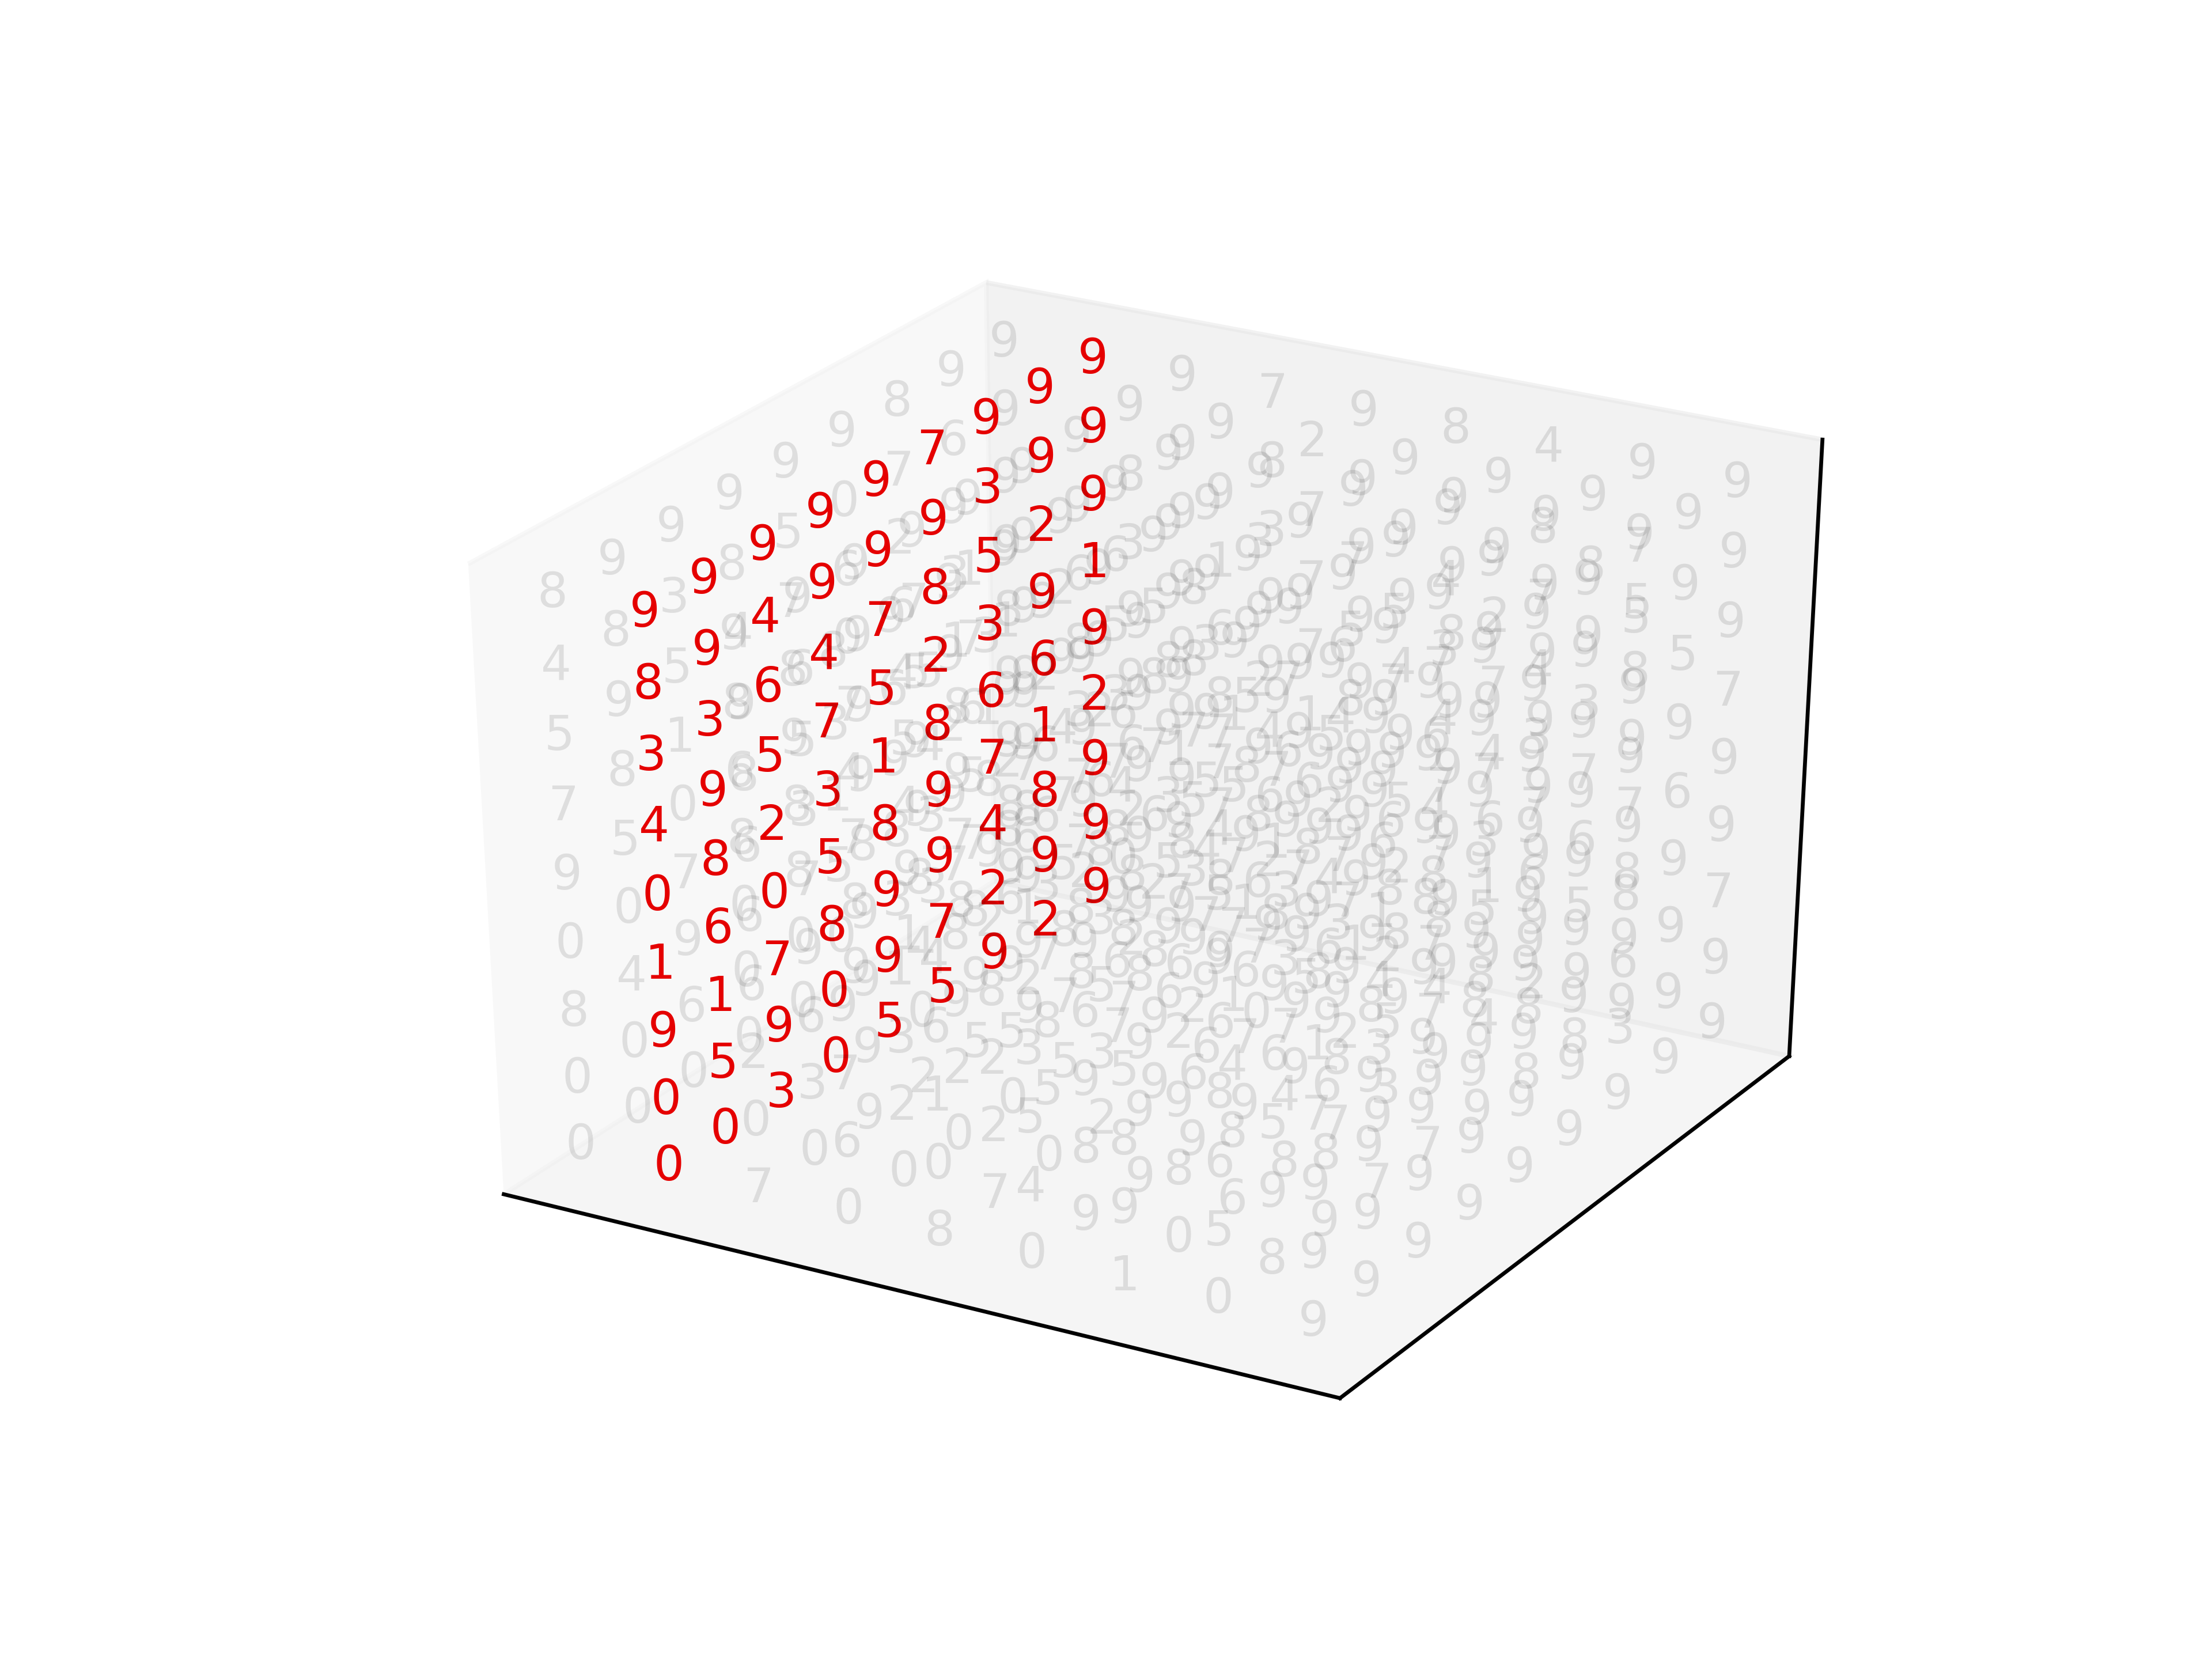
\includegraphics[width=\textwidth]{example_orientation_0}
	\end{subfigure}
	\begin{subfigure}[b]{0.4\textwidth}
		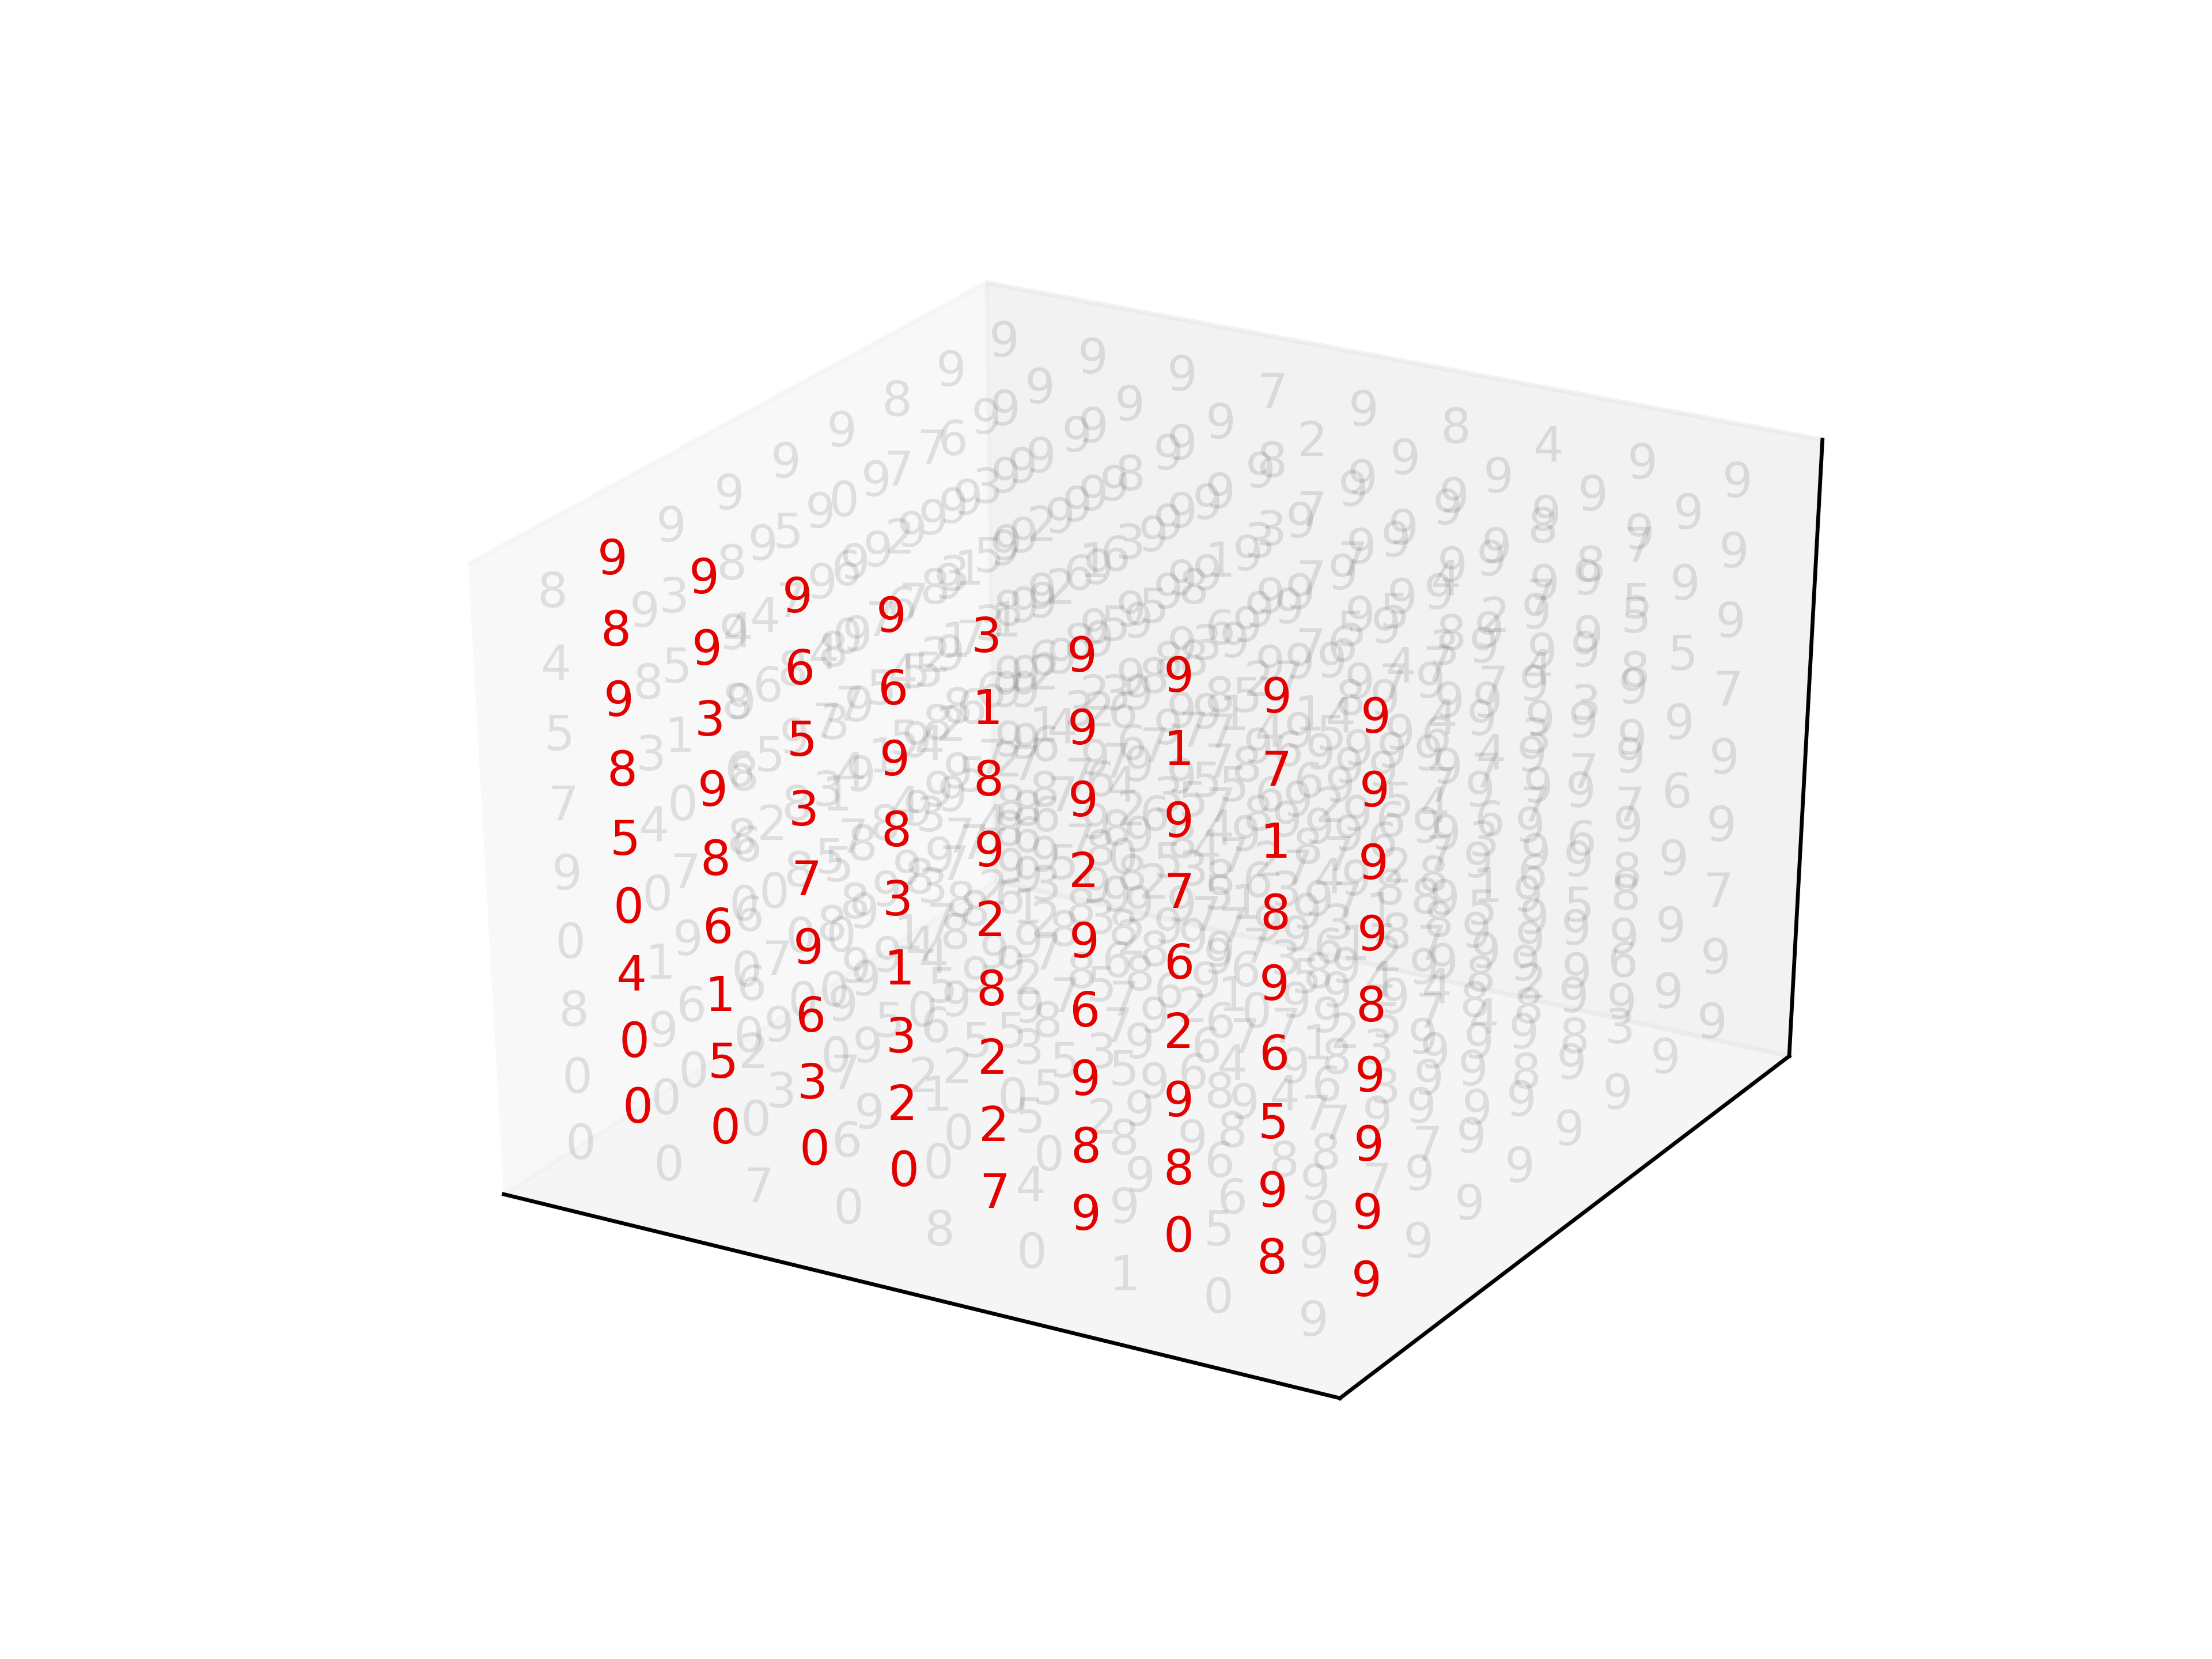
\includegraphics[width=\textwidth]{example_orientation_1}
	\end{subfigure}
	
	
	\begin{subfigure}[b]{0.4\textwidth}
		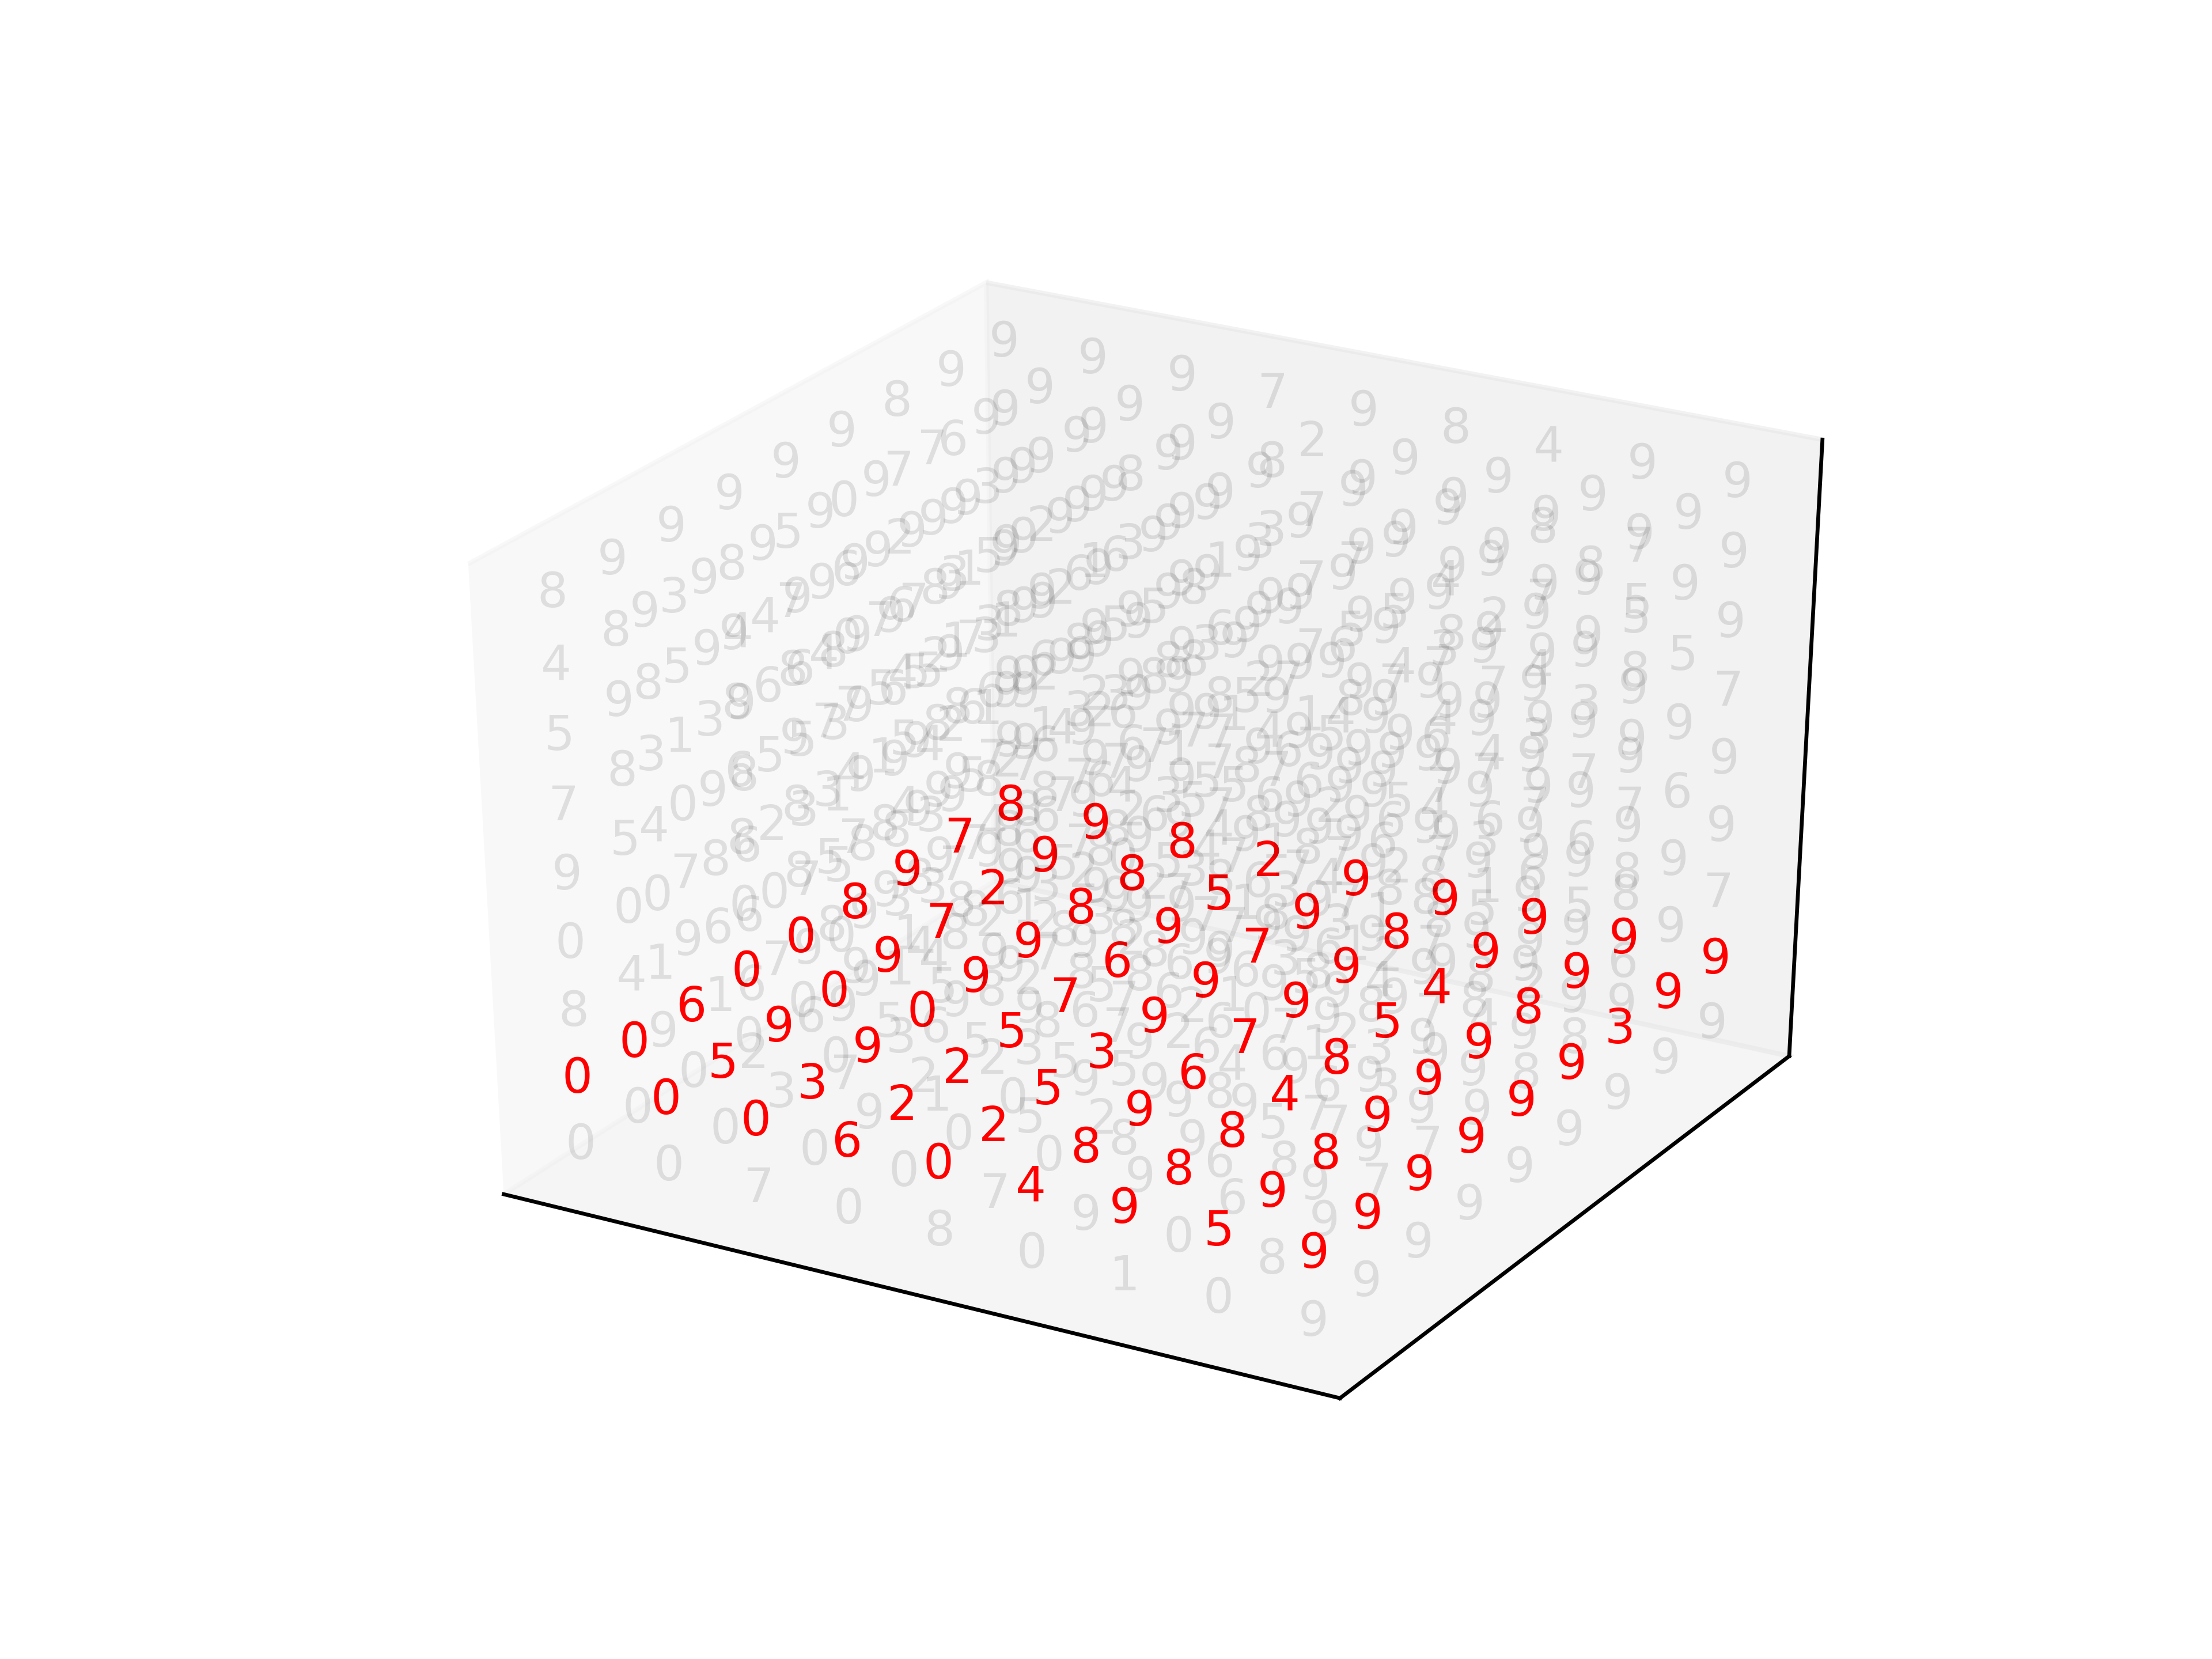
\includegraphics[width=\textwidth]{example_orientation_2}        
	\end{subfigure}
	\caption*{The 3 views of a 3D Sudoku}\label{fig:example_sudoku}
\end{figure}
\end{frame}


\begin{frame}
\frametitle{Constraints}
\begin{itemize}
\item The \texttt{digit} constraint: Only one number can be placed in a position \pause
\item The \texttt{x} direction constraint:  In the $x$ direction, all $n$ numbers should be present, and should appear exactly once \pause
\item The \texttt{y} direction constraint: In the $y$ direction, all $n$ numbers should be present, and should appear exactly once \pause
\item The \texttt{z} direction constraint: In the $z$ direction, all $n$ numbers should be present, and should appear exactly once \pause
\item The \texttt{box} constraint: In the $x$-$y$ plane, each cell of size $\sqrt{n} \times \sqrt{n}$ should contain all $n$ numbers exactly once. These cells are arranged just like the box constraint of a 2D Sudoku: $n$ boxes tiled in a $\sqrt{n} \times \sqrt{n}$ grid 
\end{itemize}
\end{frame}


\section{Hypothesis}

\begin{frame}
	\frametitle{Hypothesis}
	{\Large The \emph{relative change} in \textbf{complexity} between subsequent degrees of constraints will be the same. }	
\end{frame}


\begin{frame}
\frametitle{Dataset}

\begin{itemize}
	\item Sourced from \url{http://www.menneske.no/sudoku3d/eng/}
	\item 5354 3D Sudokus \pause
	\item Block constraint on the x-y plane 
\end{itemize}	
\end{frame}

\begin{frame}
\frametitle{SAT Solver}
{\Large PICOSAT} 
\begin{itemize}
\item Easy to use - it has \texttt{python} bindings! \pause
\item Fast \pause
\item Deterministic
\end{itemize}
\end{frame}

\begin{frame}
	\frametitle{Metric}
	{\Large The \texttt{level} metric is defined as the total number of levels divided by the number of decisions. The lower the level, the more complex the Sudoku.}
\end{frame}


\section{Encoding}  

\begin{frame}
\frametitle{Encoding}
	\begin{center}
		At Most One: $\land^{n-1}_{i=1}\land^{n}_{j=1}(\neg x_i \lor \neg x_j)$ \pause
	\end{center}
	\begin{center}
		At Least One: $\lor^{n}_{i=1}x_i$ \pause
	\end{center}
	\begin{center}
		Exactly One:  $\left(\land^{n-1}_{i=1}\land^{n}_{j=1}(\neg x_i \lor \neg x_j)\right) \land \left(\lor^{n}_{i=1}x_i\right)$
	\end{center}
\end{frame}

\section{Experimental Setup}

\begin{frame}
\frametitle{Setup - 1}

\begin{itemize}
	\item \texttt{all}: All 4 constraints were enforced
	\item \texttt{3-constraint}: Only 3 constraints out of 4 were enforced
	\item \texttt{2-constraint}: Only 2 constraints out of 4 were enforced
	\item \texttt{1-constraint}: Only 1 constraint out of 4 was enforced
\end{itemize}
\end{frame}

\begin{frame}
	\frametitle{Setup - 2}
	\begin{itemize}
	\item Ran all combinations of the constraints
	\item 15 combinations $\times$ 5354 = 80310 \pause
	\item Some puzzles time out! \pause
	\item Capped at 30 seconds of computation time
	\end{itemize}
\end{frame}

\begin{frame}
	\frametitle{Setup - 3}
	{\Large \texttt{level} metrics were then averaged per constraint combination} 
\end{frame}

\section{Results}

\begin{frame}
\frametitle{Results}
	{\small 
	\begin{table}[h]
	\begin{center}
	\setlength{\tabcolsep}{5pt}
	\begin{tabular}{| c | c | c |}
	\hline
	Constraint  & Timeouts & Average \texttt{level} \\ \hline
	\texttt{all}  & 367 &  6.507894  \\ \hline
	\texttt{x-y-block}   & 0  &  181.843220\\ \hline
	\texttt{x-z-block}  & 0 &  105.605603 \\ \hline
	\texttt{y-z-block}  & 0 &  111.127232\\ \hline
	\texttt{ x-y-z}  & 2980 &  8.734983\\ \hline
	\texttt{x-y}  & 0 &  307.721815\\ \hline
	\texttt{x-z} & 0 &  313.153474 \\ \hline
	\texttt{y-z} & 0 &  313.309301 \\ \hline
	\texttt{x-block} & 0 &  479.311524 \\ \hline
	\texttt{y-block}  & 0 &  500.234516 \\ \hline
	\texttt{z-block} & 0  &  308.272768 \\ \hline
	\texttt{x}   & 0 &  960.703399 \\ \hline
	\texttt{y}  & 0 &  960.182013 \\ \hline
	\texttt{z}   & 0 &  960.736272 \\ \hline
	\texttt{block}  & 0 &  948.700504\\ \hline
	\end{tabular}	
	\end{center}
	\end{table}
	}
\end{frame}

\begin{frame}
\frametitle{Box plot for \texttt{level}}
\begin{figure}
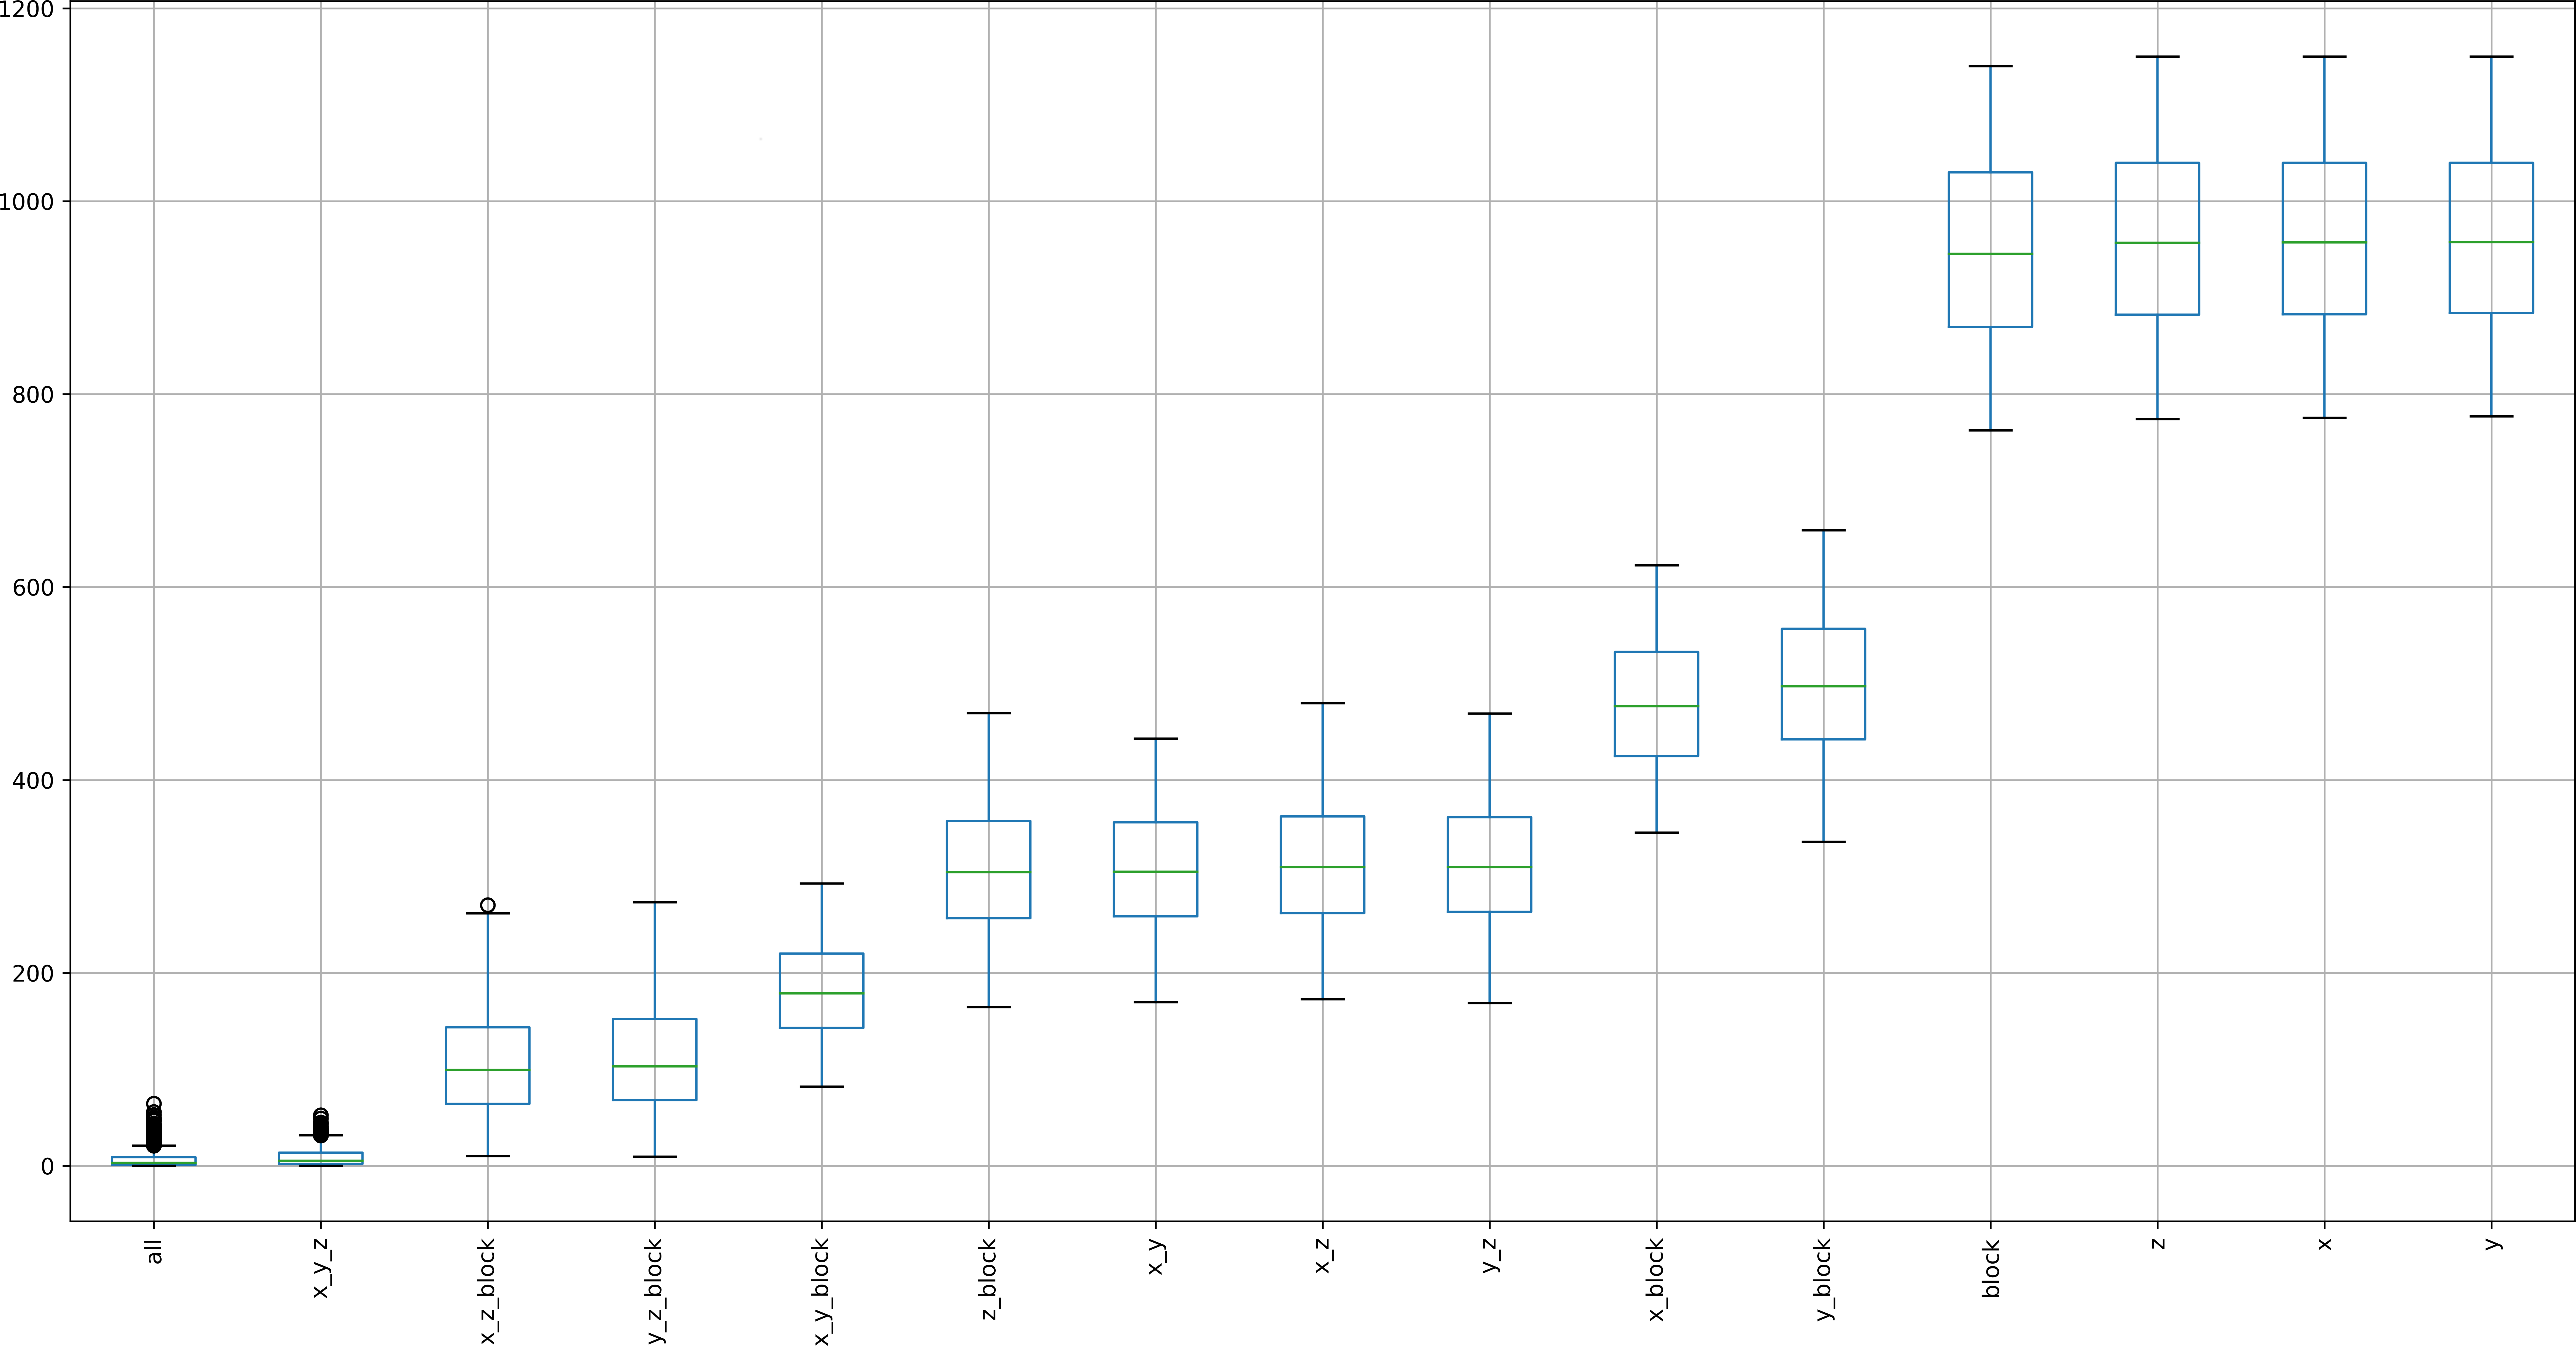
\includegraphics[width=0.9\textwidth]{level_box_plot}
\caption*{The average \texttt{level} for all constraints}
\end{figure}
\end{frame}


\begin{frame}
	\begin{figure}
		\includegraphics[scale=0.2]{error_bars}
		\caption*{Relative change in the average \texttt{level}}
	\end{figure}
\end{frame}


\section{Conclusion and Future Work}

\begin{frame}
	\frametitle{Conclusions - 1}
	{\LARGE Since there is a \alert{large variation} in these levels, we can conclude that our original hypothesis is \alert{false}}
\end{frame}

\begin{frame}
\frametitle{Conclusions - 2}
{\Large Considering the average of the \texttt{level} metrics for the 2 have overlapping uncertainty bounds, these can be considered \alert{close}} \pause \\
{\Large Considering the timeouts, the results indicate that the \alert{removal of the \texttt{block} constraint} appears to make the problem \textbf{more} difficult for the picosat solver}
\end{frame}

\begin{frame}
\frametitle{Conclusions - 3}
$\implies$ {\Large The search space is far more nuanced than we assumed \\ The most difficult constraint combination was not the combination of all of the constraints, but was found to be the combination of all 3 row constraints}
\end{frame}


\begin{frame}
\frametitle{Future Work - 1}
\begin{itemize}
\item Optimized encoding schemes \pause
\item Larger dataset \pause
\item Remove or increase runtime cap
\end{itemize}
\end{frame}

\begin{frame}
	\frametitle{Future Work - 2}
	\begin{itemize}
		\item Higher-dimensional Sudokus \pause
		\item Larger dataset \pause
		\item $>$ order \pause
		\item $<$ order  
	\end{itemize}
\end{frame}

\begin{frame}[standout]
	Thank you!
\end{frame}

 
\end{document}